\documentclass{article}
\usepackage[utf8]{inputenc}
\usepackage{graphicx}
\usepackage{listings} 
\title{Information System - Lab work 3}
\author{Tran Thi Hong Hanh}
\date{9 November 2017}

\begin{document}

\maketitle
\section*{Database}
\begin{itemize}
	\item employees (emp\_no, birth\_date, first\_name, last\_name, gender)
	\item departments (dept\_no, dept\_name)
	\item dept\_emp (emp\_no, dept\_no, from\_date, to\_date)
	\item dept\_manager (dept\_no, emp\_no, from\_date, to\_date)
	\item titles (emp\_no, title, from\_date, to\_date)
	\item salaries (emp\_no, salary, from\_date, to\_date)
\end{itemize}
\section*{SQL Queries}
\begin{enumerate}
	\item All info of all employees.\\
	
	\begin{lstlisting}[language=SQL]
SELECT * FROM employees;	
	\end{lstlisting}
	
	\item All info of all departments.\\
	
	\begin{lstlisting}[language=SQL]
SELECT * FROM departments;	
	\end{lstlisting}
	
	\item Full names of all employees.\\
	
	\begin{lstlisting}[language=SQL]
SELECT CONCAT(first_name, "", last_name) AS full_name
FROM employees;
	\end{lstlisting}
	
	\item Name of all departments\\
	
	\begin{lstlisting}[language=SQL]	
SELECT dept_name FROM departments;	
	\end{lstlisting}
	
	\item Full names of employees working in "Sale" department.\\
	
	\begin{lstlisting}[language=SQL]	
SELECT CONCAT(first_name,"", last_name) AS full_name
FROM employees
JOIN dept_emp ON employees.emp_no = dept_emp.emp_no
JOIN departments ON dept_emp.dept_no = departments.dept_no
WHERE dept_name = "Sales"
UNION
SELECT CONCAT(first_name,"", last_name) AS full_name
FROM employees
JOIN dept_manager ON employees.emp_no = dept_manager.emp_no
JOIN departments ON dept_manager.dept_no = departments.dept_no
WHERE dept_name = "Sales";
	\end{lstlisting}	
	
	\item Full names of male employees working in "Finance" department.\\
	
	\begin{lstlisting}[language=SQL]	
SELECT CONCAT(first_name, "", last_name) as full_name
FROM employees
NATURAL JOIN departments
NATURAL JOIN dept_manager
WHERE dept_name ="Finance" AND gender="M" 
UNION 
SELECT CONCAT(first_name, "", last_name) as full_name 
FROM employees
NATURAL JOIN departments 
NATURAL JOIN dept_emp
WHERE dept_name ="Finance" and gender="M" ;
	\end{lstlisting}
	
	
	\item Salaries of female employees working in "Marketing" department.\\
	
	\begin{lstlisting}[language=SQL]	
SELECT CONCAT (first_name, "", last_name) AS full_name, salary 
FROM salaries 
NATURAL JOIN employees
NATURAL JOIN departments
WHERE gender="F" AND dept_name="Marketing";
	\end{lstlisting}
	
	\item Full names of employees who have the same last name as their manager.\\
	
	\begin{lstlisting}[language=SQL]	
SELECT R1.full_name
FROM (SELECT CONCAT(first_name,"", last_name) AS full_name,
last_name, employees.emp_no AS empno 
FROM employees
JOIN dept_emp
ON employees.emp_no = dept_emp.emp_no) AS R1
JOIN (SELECT last_name, employees.emp_no AS empno 
FROM employees
JOIN dept_manager 
ON employees.emp_no = dept_manager.emp_no) AS R2
ON R1.last_name = R2.last_name;	
	\end{lstlisting}
	
	\item Full names of managers who have been doing the job at least twice.\\
	
	\begin{lstlisting}[language=SQL]	
SELECT CONCAT(first_name, "", last_name) AS full_name
FROM employees NATURAL JOIN dept_manager
GROUP BY emp_no 
HAVING count(emp_no) > 1;
	\end{lstlisting}
	
	\item Full names of employees who was paid more than \$100000.
	
	\begin{lstlisting}[language=SQL]
SELECT CONCAT(first_name, "", last_name) AS full_name, salary 
FROM employees	NATURAL JOIN salaries
WHERE salary > 100000;
	\end{lstlisting}
	
	\item Names of all departments that have employees paid more than \$100000.\\
	
	\begin{lstlisting}[language=SQL]
SELECT dept_name FROM dept_emp
NATURAL JOIN departments 
NATURAL JOIN salaries
WHERE salary > 100000
UNION
SELECT dept_name FROM departments 
NATURAL JOIN salaries 
NATURAL JOIN dept_manager
WHERE salary > 100000;
	\end{lstlisting}
\end{enumerate}

\section*{Results}

The figure below presents the results after implement 11 queries (limit from 0 to 10 for some long results
) above:\\
\begin{figure}
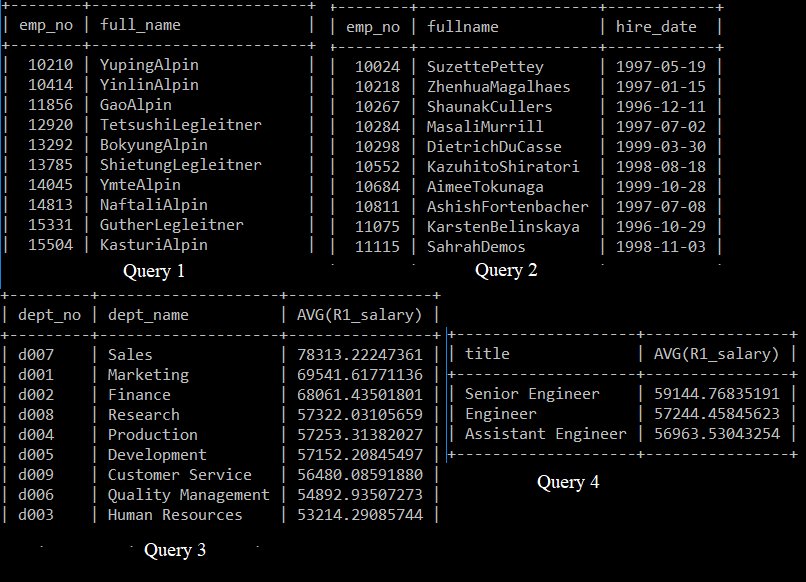
\includegraphics[scale = 0.65]{result.PNG}
\caption{Result}
\end{figure}

\end{document}
